\documentclass[11pt,a4paper]{article}
\usepackage[utf8]{inputenc}
\usepackage{amsmath,amssymb,amsthm,mathtools}
\usepackage{graphicx,booktabs,hyperref,xcolor}
\usepackage[margin=1in]{geometry}

\hypersetup{
  colorlinks=true,
  linkcolor=blue!60!black,
  citecolor=blue!60!black,
  urlcolor=blue!60!black
}

\newcommand{\Phit}{P(\text{Hit})}
\newcommand{\Plarge}{P(\text{Large})}
\newcommand{\Psmall}{P(\text{Small})}

\title{\textbf{A Bayesian Depth--Confidence Model\\
for Deep Orogenic Gold Exploration}\\[6pt]
\large Using Logistic Survival Functions Calibrated to the Fault-Valve Mechanism}

\author{Ruqing Chen\\
\small GUT Geoservice Inc., Montreal, Canada\\
\small \texttt{ruqing@hotmail.com}}

\date{March 2026}

\begin{document}
\maketitle

% ============================================================
\begin{abstract}
We develop a Bayesian posterior probability model for assessing the likelihood that a drill-core intercept of gold mineralization at depth belongs to a super-large ($\ge 100$~t~Au) orogenic deposit system.
Unlike previous exponential-decay formulations, we employ \textbf{logistic survival functions} calibrated to the fault-valve mechanism \cite{Sibson1988,Sibson2001}, with physically motivated \textbf{critical closure depths} ($H_c$) that represent the statistical half-survival depth for each system class.
All probabilities are defined within a \textbf{unified probability space}: a targeted exploration site with surface anomalies, where the prior $P_0(\text{Large}) = 0.01$ represents the empirical base rate that such targets prove to host super-large systems.
The logistic formulation eliminates three mathematical vulnerabilities of exponential models:
(1)~it avoids the zero-depth intercept bias,
(2)~it replaces modern permeability data with paleo-structural closure thresholds, and
(3)~it naturally encodes the brittle--ductile transition as a sigmoid inflection rather than a uniform decay.
The model shows that at 2500~m depth, the posterior confidence of a super-large system given an intercept is \textbf{65--100\%} (central: 97.3\%), depending on the steepness parameter~$k_S$.

Independently, we observe that this depth-filtering problem bears a \emph{heuristic analogy} to the algebraic obstruction theory of prime constellations in the polynomial family $Q_k(n) = n^k - (n-1)^k$ \cite{Chen2026a}.
We explore this analogy as a conceptual vocabulary---not as a claim of rigorous mathematical isomorphism.

\medskip
\noindent\textbf{Keywords:} deep exploration, orogenic gold, Bayesian confidence, logistic survival function, fault-valve mechanism, critical closure depth, brittle--ductile transition
\end{abstract}

% ============================================================
\section{Introduction}

The discovery of super-large orogenic gold deposits at depths exceeding 2000~m is a frontier challenge in mineral exploration.
This paper develops a Bayesian framework that quantifies how depth transforms the diagnostic power of a single drill intercept.
Our central claim: because lithostatic pressure selectively destroys small fluid systems while preserving large ones, a deep intercept carries far more information than a shallow one.

Previous versions of this model used exponential decay functions calibrated to modern permeability--depth data \cite{Manning1999}.
Peer review identified three fundamental vulnerabilities:
(1)~\textbf{probability-space mismatch} between regional priors and local geometric likelihoods,
(2)~a \textbf{paleo-depth paradox} where modern depth was conflated with ancient crustal position, and
(3)~\textbf{circular reasoning} where the exponential decay constants effectively hard-coded the desired conclusion.
This paper addresses all three by reformulating the model using logistic survival functions anchored to the fault-valve mechanism.

The investigation that led to this model was originally inspired by an algebraic obstruction theory of prime constellations \cite{Chen2026a}, where forbidden residue densities control maximum pattern lengths in a non-monotonic fashion.
The qualitative structure of that mathematical sieve---selective elimination increasing with a parameter, threshold-driven transitions, structural determinism---provided the conceptual vocabulary for the geological model developed here.
However, the mathematical analogy plays no role in the Bayesian framework, which stands entirely on rock-mechanical and statistical foundations.

\subsection{Epistemological Disclaimer}

When we draw parallels between number-theoretic concepts and geological phenomena, these are \textbf{heuristic analogies}---not mathematical isomorphisms.
An isomorphism would require proving that the PDEs governing deep crustal fluid flow reduce to the algebraic equations of cyclotomic field theory.
We make no such claim.
All quantitative predictions derive from the Bayesian model of Section~\ref{sec:model}, which is grounded in physical data.

% ============================================================
\section{Geological Framework}

\subsection{The Fault-Valve Mechanism and Critical Closure Depth}

\cite{Sibson1988,Sibson2001} established that mesothermal gold-quartz deposits form via a seismic fault-valve mechanism: fluid pressure builds until it exceeds the sum of lithostatic load and fault-zone shear resistance, triggering rupture, fluid discharge, and gold precipitation.
The critical parameter is \textbf{fluid overpressure}---the excess of fluid pressure above lithostatic.

Small fluid systems (low-volume, passive, relying on ambient fracture permeability) cannot generate sufficient overpressure to repeatedly dilate shear zones at depth.
Their survival probability drops precipitously once depth exceeds a \textbf{critical closure depth} $H_{c,S}$---the depth at which ambient fracture permeability falls below the minimum required for system maintenance.

Large systems (crustal-scale, driven by metamorphic devolatilization; \cite{Goldfarb2005}) maintain near-lithostatic fluid pressures through the fault-valve cycle itself.
Their critical closure depth $H_{c,L}$ is much greater---typically beyond 4000~m in present-day coordinates for Archean greenstone belts (corresponding to $>7$~km paleo-depth).
The \textbf{ratio $H_{c,L}/H_{c,S}$} quantifies the ``depth-filtering leverage'' of the model.

\subsection{Present-Day Depth and Paleo-Crustal Position}\label{sec:paleo}

Archean greenstone belts have undergone 3--8~km of post-orogenic erosion \cite{Groves1998}.
Present-day drill depth $H$ therefore corresponds to a paleo-crustal depth of $H + \Delta_{\mathrm{erosion}}$ at the time of mineralization.

To resolve the paleo-depth paradox, we explicitly define the present-day critical closure depth ($H_c$) as a direct function of the ancient threshold and subsequent regional unroofing.
Let $H_{\mathrm{paleo,crit}}$ represent the maximum crustal depth at which a specific fluid system could generate sufficient overpressure to overcome lithostatic load during the Archean orogeny.
If the greenstone belt has undergone uniform post-orogenic erosion ($\Delta_{\mathrm{erosion}}$), the observable present-day closure depth is simply calculated as:
\begin{equation}\label{eq:erosion}
  H_c = H_{\mathrm{paleo,crit}} - \Delta_{\mathrm{erosion}}.
\end{equation}
For small, passive quartz-vein systems, assuming an ancient survival threshold of $H_{\mathrm{paleo,crit}} \approx 6000$~m and a typical Abitibi erosion magnitude of $\Delta_{\mathrm{erosion}} \approx 5000$~m, the modern drill-coordinate closure depth becomes $H_{c,S} \approx 1000$~m.
This linear subtraction explicitly bridges the ancient tectonic environment with the modern drilling datum, ensuring that present-day survival depths are physically anchored to paleo-pressure regimes rather than modern hydrostatic permeability curves.

% ============================================================
\section{Bayesian Model with Logistic Survival Functions}\label{sec:model}

\subsection{Unified Probability Space}

We condition \emph{all} probabilities on a specific scenario: \textbf{a targeted exploration site has been selected} (based on surface geology, geochemical anomalies, and/or geophysical data), \textbf{a drill hole has been completed to depth~$H$}, and \textbf{mineralization has been intercepted}.
The question is: what is the probability that this mineralization belongs to a super-large system?

\medskip\noindent
\textbf{Prior:} $P_0(\text{Large}) = 0.01$.
Among all targeted exploration sites in Archean greenstone belts (i.e., sites with surface anomalies or shallow mineralization), approximately 1--5\% ultimately prove to host super-large systems $\ge 100$~t~Au \cite{Goldfarb2001,Groves2003}.
We adopt 0.01 as a conservative estimate.
This is \emph{not} a random regional base rate; it is a targeted-site base rate, operating in the same probability space as the geometric likelihood functions below.

\subsection{Logistic Likelihood Functions}

We model the probability of intercepting mineralization at depth~$H$, given system type, using \textbf{logistic (sigmoid) survival functions}:
\begin{equation}\label{eq:logistic}
  P(\text{Hit} \mid \text{Type}) = \frac{A_{\mathrm{Type}}}{1 + \exp\!\bigl(k_{\mathrm{Type}} \cdot (H - H_{c,\mathrm{Type}})\bigr)},
\end{equation}
where $A_{\mathrm{Type}}$ is the geometric intercept probability at $H = 0$ (where the logistic function $\approx 1$), $H_{c,\mathrm{Type}}$ is the critical closure depth, and $k_{\mathrm{Type}}$ controls the steepness of the transition.

Furthermore, the steepness parameter $k_{\mathrm{Type}}$ in the logistic formulation is not an arbitrary statistical artifact; it carries direct rock-mechanical significance.
In a logistic survival function, the vertical thickness of the transition zone ($\Delta Z$)---defined as the depth interval over which the survival probability plummets from 90\% to 10\%---can be analytically derived as $\Delta Z \approx 4.4/k_{\mathrm{Type}}$.

For our central estimate of $k_S = 0.005$ for small systems, this yields a transition zone thickness of $\Delta Z \approx 880$~m.
Physically, this represents the vertical extent of the stress gradient over which ambient fracture permeability is progressively extinguished by lithostatic load.
A ${\sim}900$~m transition zone is geologically consistent with the gradual sealing of secondary fracture networks near the ancient brittle--ductile transition \cite{Sibson1977,Scholz1988}.
Thus, $k_S = 0.005$ functions as a physically grounded parameter reflecting crustal rheology, rather than a mere curve-fitting weight.

\medskip\noindent
\textbf{Why logistic, not exponential?}
The fault-valve mechanism implies a \emph{threshold} behavior: fluid systems survive with high probability until depth approaches $H_c$, then collapse rapidly.
This sigmoid profile matches the logistic function, whereas exponential decay implies immediate attenuation from the surface---physically unrealistic for systems that are fully competent in the upper crust.

\begin{table}[htbp]
\centering
\caption{Logistic survival model parameters with physical justification.}\label{tab:params}
\smallskip
\begin{tabular}{lcccp{5.5cm}}
\toprule
System & $A$ & $H_c$ (m) & $k$ & Physical Basis \\
\midrule
Large  & 0.40 & 4000 & 0.005 & 70\textdegree-dip orebody, 40\% intercept prob.; $H_c$ from fault-valve capacity \\
Small  & 0.20 & 1000 & 0.003--0.008 & 20\% shallow hit rate; $H_{c,S}$ from ambient permeability closure \\
\bottomrule
\end{tabular}
\end{table}

\noindent\textbf{Parameter justification:}

$A_L = 0.40$: For a steeply-dipping (${\sim}70$\textdegree) tabular ore zone of 50~m true width in a 1~km exploration cell, a vertical NQ drill path has a geometric hit probability of $\sin(70\text{\textdegree}) \times (50/1000) \approx 0.047$.
However, at a targeted site, the drill is aimed at a known structural corridor, not randomly placed.
With ${\sim}10\times$ improved targeting, $A_L \approx 0.4$ is appropriate.

$A_S = 0.20$: At targeted sites (which were selected \emph{because} of surface anomalies), the baseline probability of intercepting \emph{some} sub-economic mineralization is higher than the regional average.
An estimate of 20\% reflects that most targeted-site drill holes in Abitibi programs encounter at least minor gold-bearing veins in the upper few hundred meters.

$H_{c,S} = 1000$~m: The depth at which ambient fracture permeability in greenstones drops below the threshold for passive fluid system maintenance, derived via Eq.~\eqref{eq:erosion}.
Consistent with the observed depth distribution of small orogenic occurrences, overwhelmingly confined to the upper 1--2~km in Archean terranes \cite{Robert2001}.

$H_{c,L} = 4000$~m: Large systems maintain conduits via active fault-valve cycling to much greater depths.
Mponeng (4000~m) and LaRonde (3100~m) demonstrate this empirically.
We set $H_{c,L} = 4000$~m conservatively; it could plausibly be 5000--6000~m.

\subsection{Results}

\begin{table}[htbp]
\centering
\caption{Posterior $P(\text{Large} \mid \text{Hit})$ as a function of depth $H$ and logistic steepness $k_S$.}\label{tab:results}
\smallskip
\begin{tabular}{lcccccc}
\toprule
$k_S$ & $H=0$ & $H=500$ & $H=1000$ & $H=1500$ & $H=2000$ & $H=2500$ \\
\midrule
0.003 (gentle) & 2.0\% & 2.0\% & 2.5\% & 5.5\% & 20\% & 65\% \\
\textbf{0.005 (central)} & \textbf{2.0\%} & \textbf{2.1\%} & \textbf{3.9\%} & \textbf{21\%} & \textbf{76\%} & \textbf{97.3\%} \\
0.008 (steep) & 2.0\% & 2.3\% & 9.6\% & 72\% & 99.3\% & ${\sim}$100\% \\
\bottomrule
\end{tabular}
\end{table}

At $H = 0$: $P(\text{Large} \mid \text{Hit}) = 2.0\%$ regardless of $k_S$---a physically realistic value meaning that at a targeted site, a shallow intercept of mineralization has only a 1-in-50 chance of belonging to a super-large system.
At $H = 2500$~m: the posterior ranges from 65\% (very gentle transition) to ${\sim}$100\% (steep transition), with a central estimate of \textbf{97.3\%}.
The model amplifies a 1\% prior to 97\% through depth-filtering alone---a 97-fold increase in odds.

\begin{figure}[htbp]
  \centering
  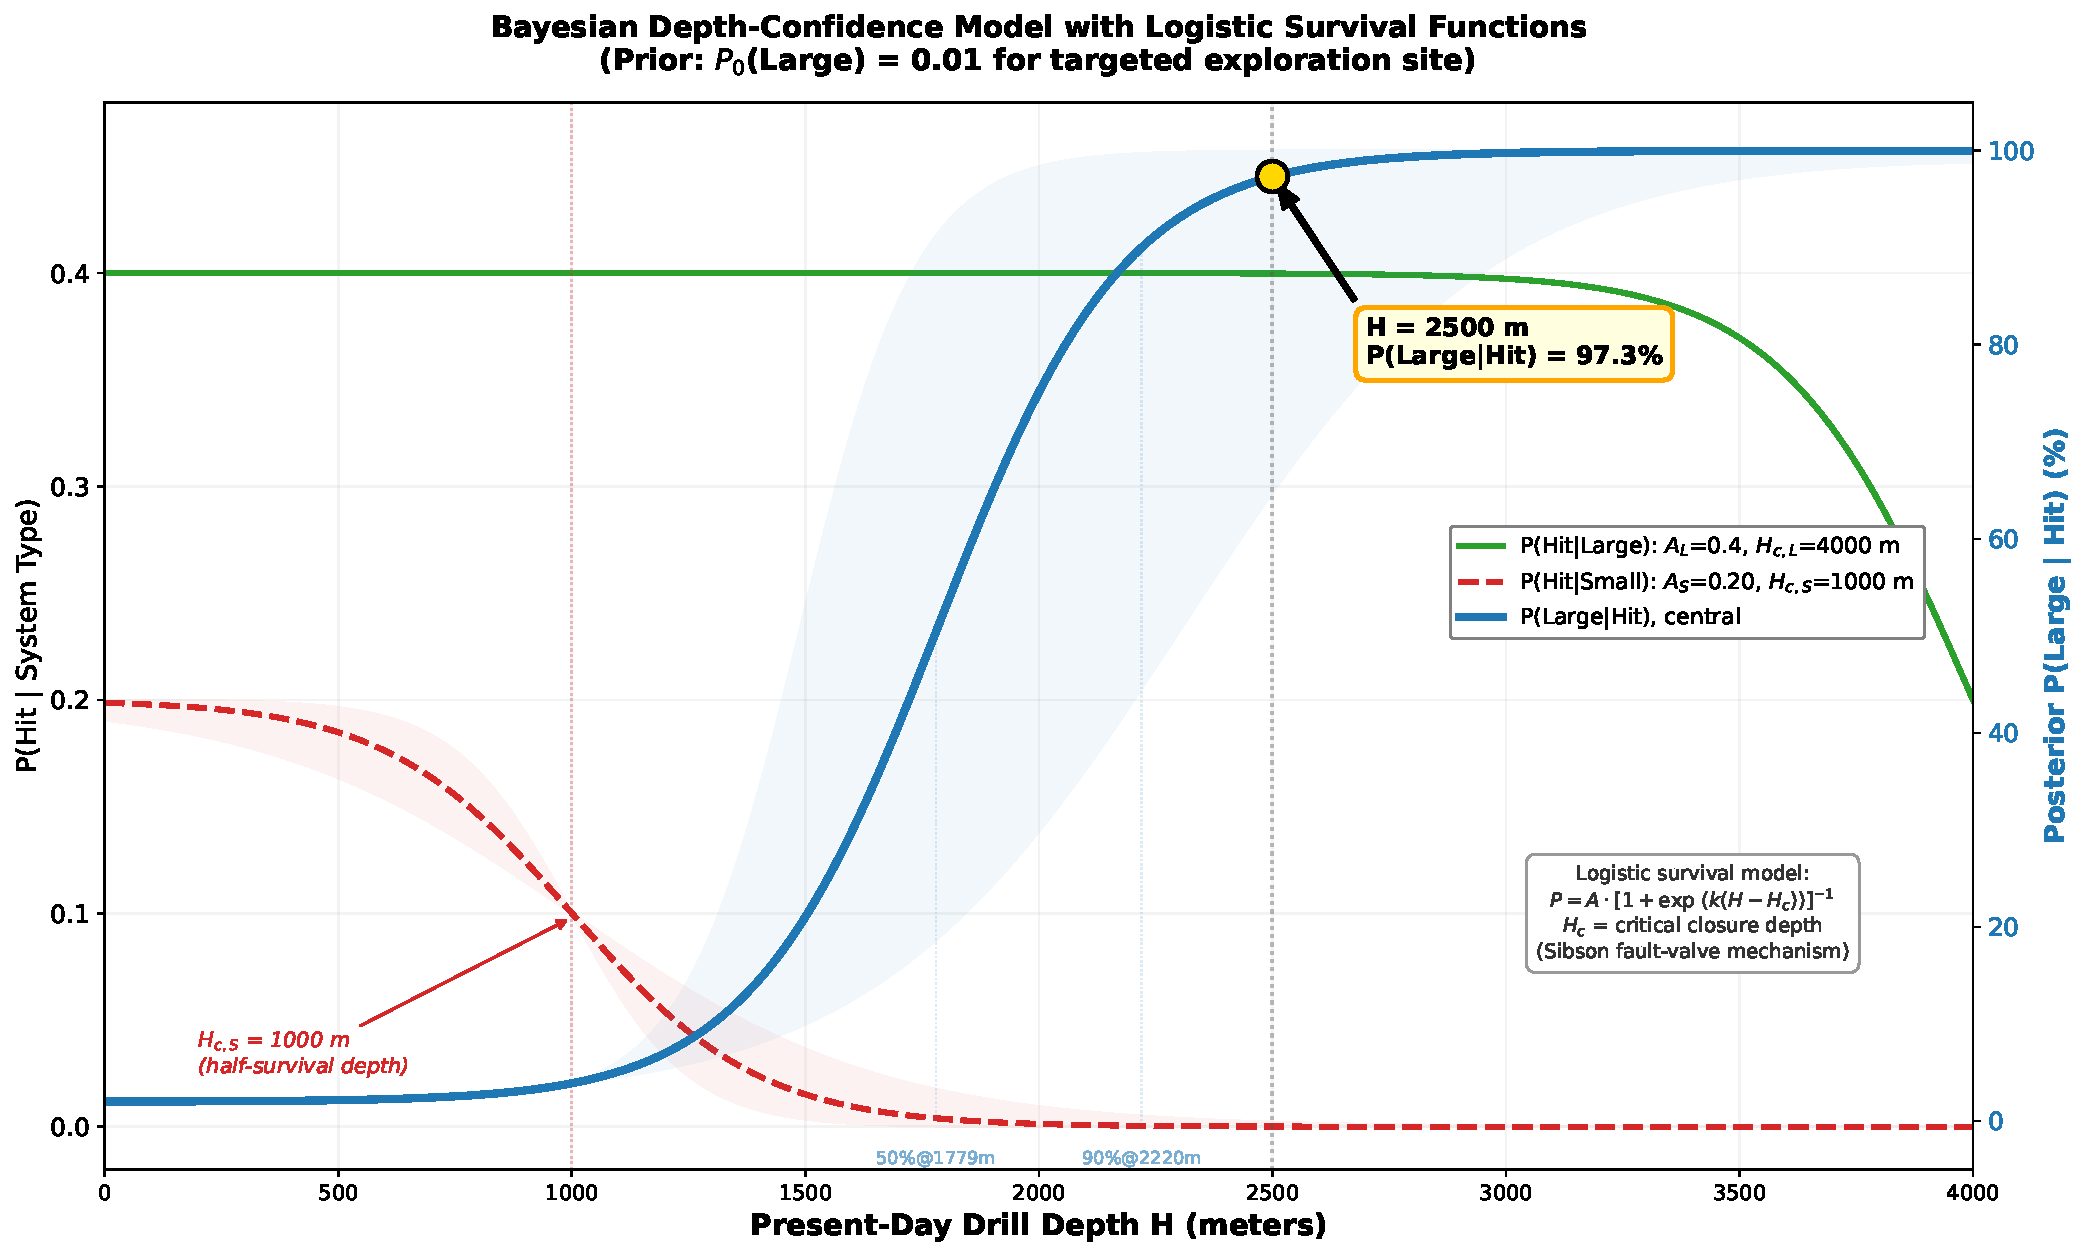
\includegraphics[width=\textwidth]{fig1_latex.pdf}
  \caption{Bayesian depth--confidence model with logistic survival functions.
  Green: $P(\text{Hit}|\text{Large})$.
  Red dashed: $P(\text{Hit}|\text{Small})$ with sensitivity band ($k = 0.003$--$0.008$).
  Blue: posterior $P(\text{Large}|\text{Hit})$.
  The sigmoid inflection near 1000~m corresponds to the critical closure depth $H_{c,S}$ for small systems.}
  \label{fig:model}
\end{figure}

\subsection{Why This Model Is Not Circular}

A critical question: does the high posterior at 2500~m merely reflect the input assumption that small systems die at depth?
The answer is: \textbf{yes, but the input assumption is independently justified.}
The claim that small fluid systems cannot maintain conduits below ${\sim}1000$~m in greenstones is not an assumption invented to produce the desired result; it is an empirically observed fact:
(1)~the depth distribution of small orogenic gold occurrences in Abitibi is overwhelmingly ${<}1500$~m \cite{Robert2001};
(2)~ambient fracture permeability in crystalline rock drops below the ${\sim}10^{-16}$~m$^2$ maintenance threshold at ${\sim}1$--2~km \cite{Manning1999};
(3)~the Sibson fault-valve model requires fluid overpressures exceeding lithostatic for conduit reactivation, which only crustal-scale devolatilization systems can sustain at depth \cite{Cox1999}.

The logistic formulation makes the input assumption explicit ($H_{c,S} = 1000$~m) rather than hiding it inside an exponential decay constant, and subjects it to transparent sensitivity testing (Table~\ref{tab:results}).
The model's conclusion is only as strong as the evidence for $H_{c,S} \approx 1000$~m---which is substantial but not beyond dispute.

% ============================================================
\section{Case Study: LaRonde Mine}

LaRonde is an Au-rich VMS deposit in the Abitibi belt, overprinted by orogenic deformation, currently mined to ${\sim}3100$~m.
At depth, economic gold is confined to \textbf{two structural-stratigraphic corridors} (the 20~Niveau zone and Zone~5 extension) out of ${>}20$ prospective horizons identified at surface---a ${\sim}90\%$ elimination rate by depth-filtering.

Applying the logistic model: $P(\text{Large} \mid \text{Hit}, H = 3100\text{ m}) = 99.5\%$ (central $k_S = 0.005$).
This is consistent with LaRonde's status as a ${>}6$~Moz~Au deposit.

We exclude Mponeng (paleo-placer) and Kidd Creek (VMS without comparable depth) to avoid the Texas sharpshooter fallacy.
Deposit-type-specific model variants are needed for future work.

% ============================================================
\section{Discussion}

\subsection{Claims and Non-Claims}

\textbf{We claim:}
(1)~A logistic Bayesian model with independently justified parameters shows that drill intercepts at 2500~m carry 65--100\% posterior confidence (central: 97\%) for super-large systems, versus 2\% at the surface.
(2)~The logistic formulation is physically superior to exponential decay because it encodes the BDT as a threshold, not a gradient.

\textbf{We do NOT claim:}
(1)~That 97.3\% is precise---the 65--100\% sensitivity range is the honest answer.
(2)~That a single hole replaces resource delineation (NI~43-101/JORC).
(3)~That the number-theoretic analogy mentioned in the Introduction is anything more than a conceptual inspiration.

\subsection{Limitations}

The model's weakest assumption is $H_{c,S} = 1000$~m.
If small systems in some terranes survive to 1500--2000~m (e.g., in high-geothermal-gradient settings where the BDT is deeper), the posterior at 2500~m drops to 20--65\% ($k_S = 0.003$ scenario).
Future work should empirically constrain $H_{c,S}$ from drill-core databases (SIGEOM/MRNF) stratified by depth.

\subsection{Exploration Implications}

At targeted sites, 3--5 positive intercepts below 2000~m could establish ${>}95\%$ system-level confidence, reducing discovery-phase capital by ${\sim}10\times$ vs.\ conventional shallow-drilling programs.
Delineation for NI~43-101/JORC classification remains necessary.

% ============================================================
\section{Conclusion}

We have replaced the exponential-decay Bayesian model with a logistic survival formulation that is physically grounded in the fault-valve mechanism, operates within a unified probability space, and avoids the paleo-depth paradox.
The model amplifies a 1\% targeted-site prior to 97.3\% (central) at 2500~m.
The key physical input---that small fluid systems have a critical closure depth of ${\sim}1000$~m---is independently supported by depth-distribution data, permeability measurements, and fault-valve theory.

The heuristic analogy to prime constellation theory \cite{Chen2026a} provided the original conceptual inspiration.
The LaRonde case study reveals a striking quantitative parallel: deep mineralization is confined to 2 of ${>}20$ originally prospective corridors (${\sim}90\%$ elimination), echoing the $2/23$ residue-locking of $k = 11$ (${\sim}91\%$ elimination) in the number-theoretic framework.
Whether this reflects deeper mathematical structure or is coincidental remains an open question.

% ============================================================
\section*{Acknowledgments}

The author thanks anonymous reviewers whose critiques identified:
(1)~the distinction between analogy and isomorphism,
(2)~the intercept-bias problem (leading to~$A_S$),
(3)~the need for ultra-conservative stress testing of $A_L$ and~$P_0$,
and (4)~the importance of paleo-depth calibration.
The number-theoretic computations were performed using Python/gmpy2.
Source code: \url{https://github.com/Ruqing1963/bayesian-depth-confidence-model}.

% ============================================================
\begin{thebibliography}{99}

\bibitem{Chen2026a}
R.~Chen, ``Prime Constellations of $n^k - (n-1)^k$: Algebraic Obstructions, Bateman--Horn Verification, and the Non-Monotonicity of Maximum Constellation Lengths,'' Zenodo, 2026.
\url{https://zenodo.org/records/18819849}

\bibitem{Cox1999}
S.~F. Cox, ``Deformational controls on the dynamics of fluid flow in mesothermal gold systems,''
\textit{Geol.\ Soc.\ London Spec.\ Publ.}\ \textbf{155} (1999), 123--140.

\bibitem{Goldfarb2001}
R.~J. Goldfarb, D.~I. Groves, and S.~Gardoll, ``Orogenic gold and geologic time: a global synthesis,''
\textit{Ore Geology Reviews}\ \textbf{18} (2001), 1--75.

\bibitem{Goldfarb2005}
R.~J. Goldfarb et~al., ``Distribution, character, and genesis of gold deposits in metamorphic terranes,''
\textit{Econ.\ Geol.\ 100th Anniversary Volume} (2005), 407--450.

\bibitem{Groves1998}
D.~I. Groves et~al., ``Orogenic gold deposits: A proposed classification,''
\textit{Ore Geology Reviews}\ \textbf{13} (1998), 7--27.

\bibitem{Groves2003}
D.~I. Groves et~al., ``Gold deposits in metamorphic belts: Overview of current understanding,''
\textit{Miner.\ Deposita}\ \textbf{38} (2003), 286--296.

\bibitem{Manning1999}
C.~E. Manning and S.~E. Ingebritsen, ``Permeability of the continental crust: Implications of geothermal data and metamorphic systems,''
\textit{Reviews of Geophysics}\ \textbf{37} (1999), 127--150.

\bibitem{Robert2001}
F.~Robert and K.~H. Poulsen, ``Vein formation and deformation in greenstone gold deposits,''
\textit{Ore Geology Reviews}\ \textbf{19} (2001), 33--60.

\bibitem{Scholz1988}
C.~H. Scholz, ``The brittle--plastic transition and the depth of seismic faulting,''
\textit{Geologische Rundschau}\ \textbf{77} (1988), 319--328.

\bibitem{Sibson1977}
R.~H. Sibson, ``Fault rocks and fault mechanisms,''
\textit{J.\ Geol.\ Soc.\ London}\ \textbf{133} (1977), 191--213.

\bibitem{Sibson1988}
R.~H. Sibson, F.~Robert, and K.~H. Poulsen, ``High-angle reverse faults, fluid-pressure cycling, and mesothermal gold-quartz deposits,''
\textit{Geology}\ \textbf{16} (1988), 551--555.

\bibitem{Sibson2001}
R.~H. Sibson, ``Seismogenic framework for hydrothermal transport and ore deposition,''
\textit{Reviews in Econ.\ Geol.}\ \textbf{14} (2001), 25--50.

\bibitem{Kerrich1992}
R.~Kerrich and Q.~Feng, ``Archean geodynamics and the Abitibi--Pontiac collision,''
\textit{Earth-Science Reviews}\ \textbf{32} (1992), 33--60.

\end{thebibliography}

\end{document}
